\chapter{Requirement Analysis}
\section{Ardunio}
\begin{figure}[H]
 \centering
    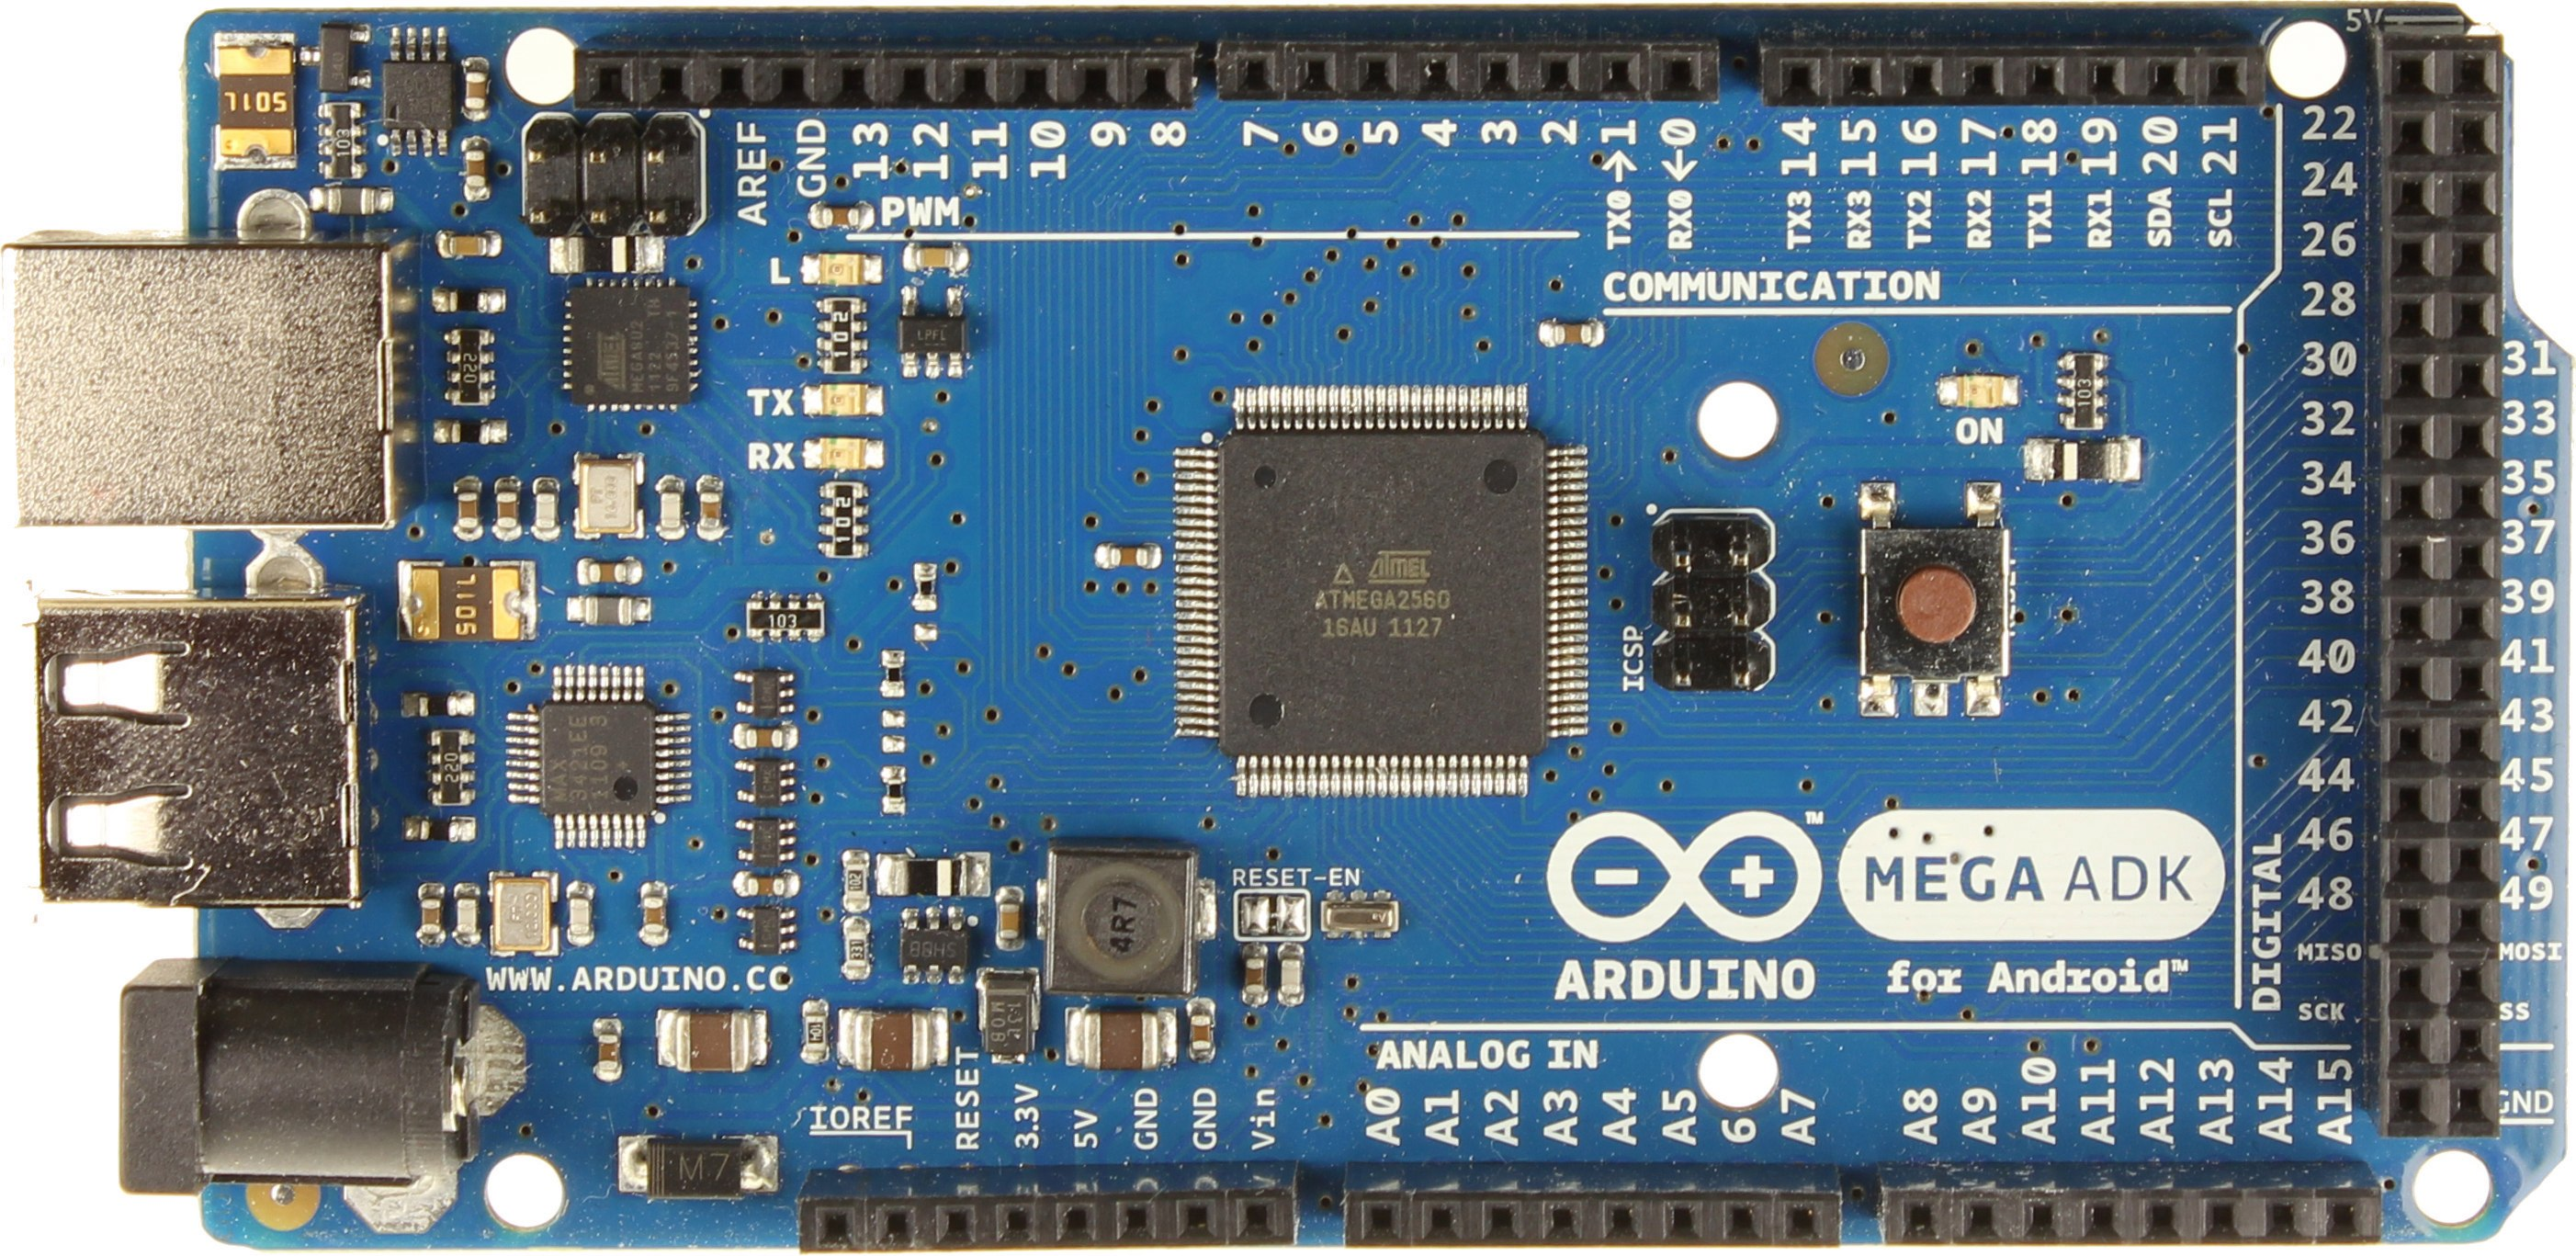
\includegraphics[height= 4cm, width=7cm]{project/images/ardunio}
  \caption{\textbf{Ardunio MEGA ADK}}
\end{figure}
\paragraph{}The Arduino Mega is a microcontroller board based on the ATmega1280 (datasheet). It has 54 digital input/output pins (of which 14 can be used as PWM outputs), 16 analog inputs, 4       UARTs (hardware serial ports), a 16 MHz crystal oscillator, a USB connection, a power jack, an ICSP header, and a reset button. It contains everything needed to support the microcontroller; simply connect it to a computer with a USB cable or power it with a AC-to-DC adapter or battery to get started. The Mega is compatible with most shields designed for the Arduino Duemilanove or Diecimila.
\large{\textbf{\\SUMMARY OF ARDUNIO}} 
\begin{enumerate}[a. ]
 \item Microcontroller ATmega1280
 \item Operating Voltage	5V
\item Input Voltage (recommended)	7-12V
\item Input Voltage (limits)	6-20V
\item Digital I/O Pins	54 (of which 15 provide PWM output)
\item Analog Input Pins	16
\item DC Current per I/O Pin	40 mA
\item DC Current for 3.3V Pin	50 mA
\item Flash Memory	128 KB of which 4 KB used by bootloader
\item SRAM	8 KB
\item EEPROM	4 KB
\item Clock Speed	16 MHz

\end{enumerate}

\section{Lazer}
\begin{figure}[H]
 \centering
    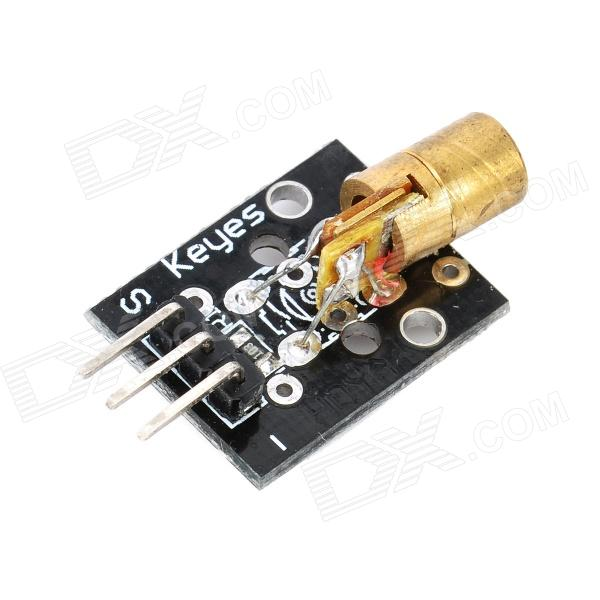
\includegraphics[height= 4cm, width=7cm]{project/images/lazer}
  \caption{\textbf{REES52 6 Psc Lazer}}
\end{figure}
\paragraph{}A laser is a device that emits light through a process of optical amplification based on the  stimulated  emission  of  electromagnetic  radiation.  The  term  "laser"  originated  as  an acronym for "light amplification by stimulated emission of radiation".
A laser differs from other sources of light in that it emits light coherently. Spatial coherence allows a laser to be focused to a tight spot, enabling applications such as laser cutting and lithography. Spatial coherence also allows a laser beam to stay narrow over great distances (collimation), enabling applications such as laser pointers. Lasers can also have high temporal coherence, which allows them to emit light with a very narrow spectrum, i.e., they can emit a single colour of light. Temporal coherence can be used to produce pulses of light as short as a femtosecond.


\section{GSM Module}

\begin{figure}[H]
 \centering
    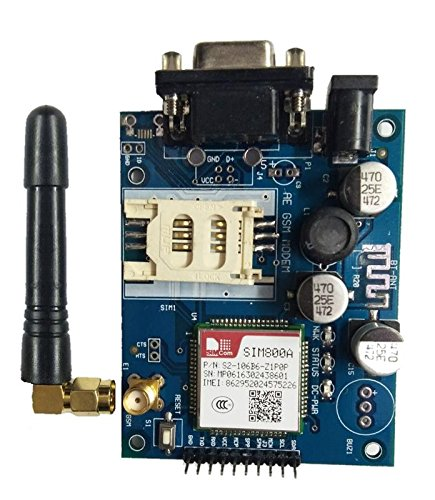
\includegraphics[height= 4cm, width=7cm]{project/images/sim module}
  \caption{\textbf{SIM 900}}
\end{figure}
\paragraph{}A GSM Module is basically a GSM Modem (like SIM 900) connected to a PCB with different types of output taken from the board – say TTL Output (for Arduino, 8051 and other microcontrollers) and RS232 Output to interface directly with a PC (personal computer). The board will also have pins or provisions to attach mic and speaker, to take out +5V or other values of power and ground connections. These type of provisions vary with different modules.Lots of varieties of GSM modem and GSM Modules are available in the market to choose from. For our project of connecting a gsm modem or module to arduino and hence send and receive sms using arduino – its always good to choose an arduino compatible GSM Module – that is a GSM module with TTL Output provisions.

\section{LDR}
\begin{figure}[H]
 \centering
    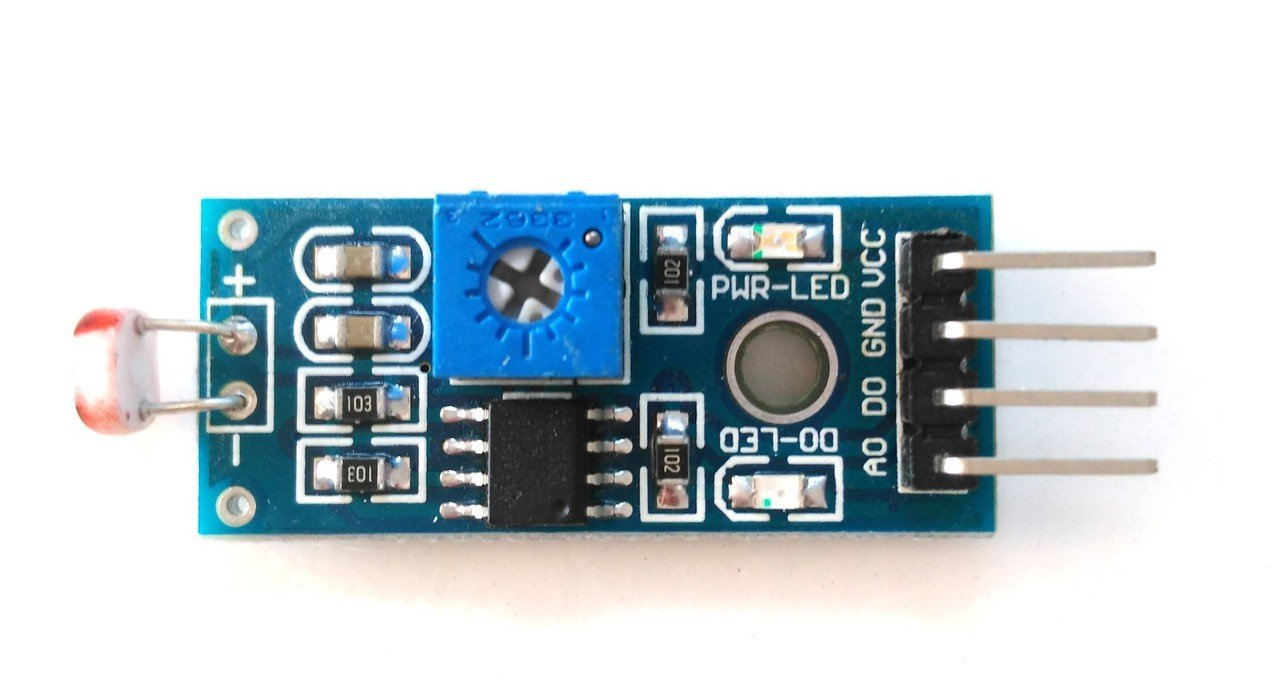
\includegraphics[height= 4cm, width=7cm]{project/images/LDR}
  \caption{\textbf{LDR}}
\end{figure}
\paragraph{}A Light Dependent Resistor (also known as a photoresistor or LDR) is a device whose resistivity is a function of the incident electromagnetic radiation. Hence, they are light-sensitive devices. They are also called as photoconductors, photoconductive cells or simply photocells.They are made up of semiconductor materials that have high resistance. There are many different symbols used to indicate a photoresistor or LDR, one of the most commonly used symbol is shown in the figure below. The arrow indicates light falling on it.Those semiconductor materials which have a direct band gap are the ones that emit photons. When a suitable voltage is applied to the leads, electrons are able to recombine with electron holes within the device, releasing energy in the form  of  photons.  This  effect  is called  electroluminescence  and  the  colour  of  the  light (corresponding to the energy of the photon) is determined by the energy band gap of the semiconductor. An LED is often small in area (less  than I mm2) and integrated optical components may be used to shape its radiation pattern

\section{Buzzer}
\begin{figure}[H]
 \centering
    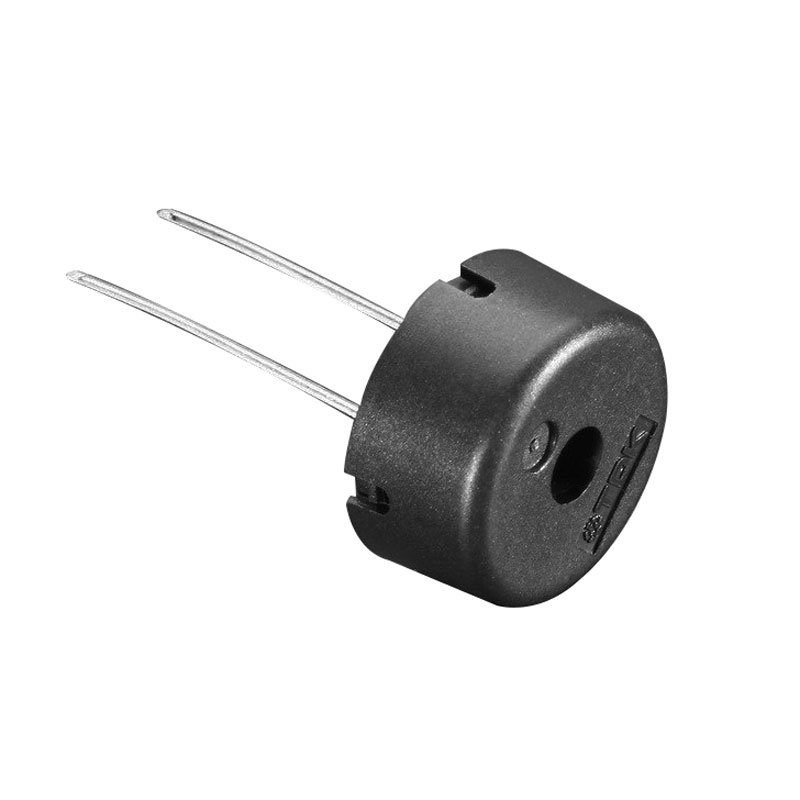
\includegraphics[height= 4cm, width=7cm]{project/images/buzzer}
  \caption{\textbf{buzzer}}
\end{figure}
\paragraph{}A  buzzer  or  beeper  is  an  audio  signalling  device,  which  may  be  mechanical, electromechanical, and piezoelectric. Typical uses of buzzers and beepers  include  alarm devices, timers and confirmation of user input such as a mouse click or keystroke.
Early devices were based on an electromechanical system identical to an electric bell without the metal gong. Similarly, a relay may be connected to interrupt its own actuating current, causing the contacts to buzz. Often these units were anchored to a wall or ceiling to use it as a sounding board. The word "buzzer" comes from the rasping noise that electromechanical buzzers made.
The buzzer consists of an outside case with two pins to attach it to power and ground.  When current is applied to the buzzer it causes the ceramic disk to contract or expand. Changing this then causes the surrounding disc to vibrate. That's the sound that you hear. Adjust the potentiometer to increase or decrease the resistance of the potentiometer. If you increase the resistance of the potentiometer then it will decrease the Volume of the buzzer. If you decrease the resistance of the potentiometer then it will increase the Volume of the buzzer.

